\begin{figure*}
\centering

\setlength{\tabcolsep}{1pt}
{\small
\begin{tabular}{c c c c c c c c c}
    & \multicolumn{2}{c}{``A Gundam''} & { } & \multicolumn{2}{c}{``A tank''} & { } & \multicolumn{2}{c}{``A glass and metal battle-axe''} \\
    %
    \raisebox{20pt}{\rotatebox[origin=c]{90}{Input}} &
    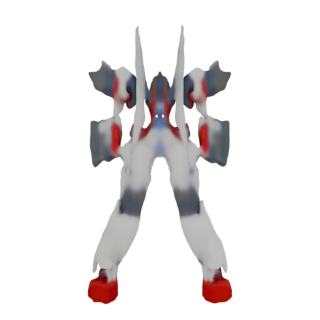
\includegraphics[width=0.13\linewidth]{images/generation_results/shap-e/gundam/gundam_tile_1.png} &
    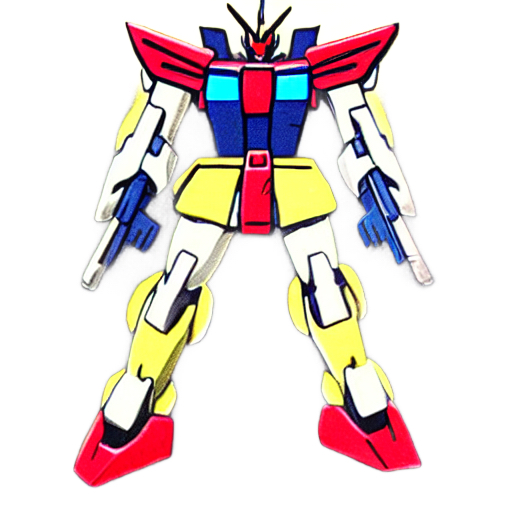
\includegraphics[width=0.13\linewidth]{images/generation_results/zero123/gundam/gundam_solo.jpg} & { } & 
    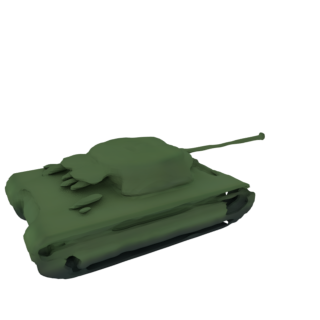
\includegraphics[width=0.13\linewidth, trim=0 0 0 60, clip]{images/generation_results/shap-e/tank/tank_tile_2.png} &
    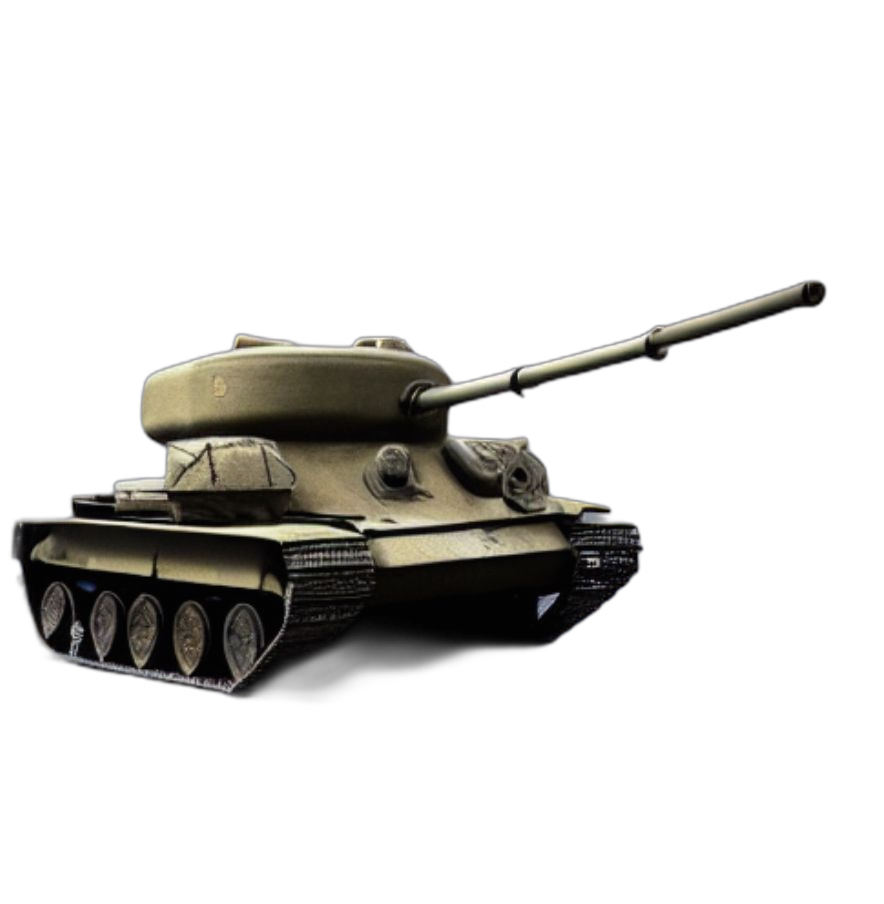
\includegraphics[width=0.13\linewidth, trim=0 50 0 150, clip]{images/generation_results/zero123/tank/tank_rem.jpg} & { } & 
    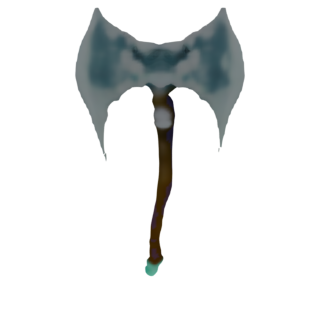
\includegraphics[width=0.13\linewidth]{images/generation_results/shap-e/glass_battle_axe/glass_battle_axe_tile_4.png} &
    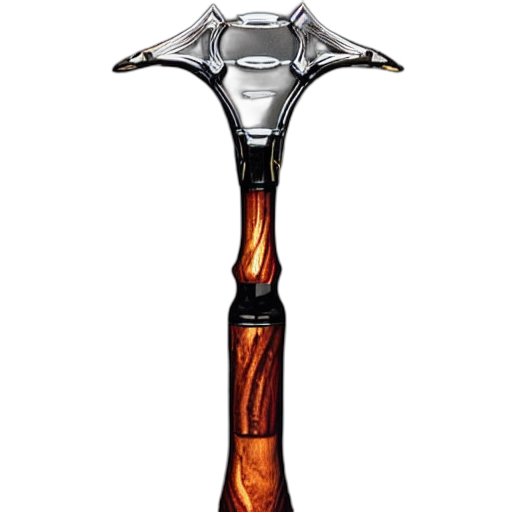
\includegraphics[width=0.13\linewidth]{images/generation_results/zero123/glass_axe/glass_axe_14_rem.jpg}
    \\
    %
      \raisebox{20pt}{\rotatebox[origin=c]{90}{View 1}} &
    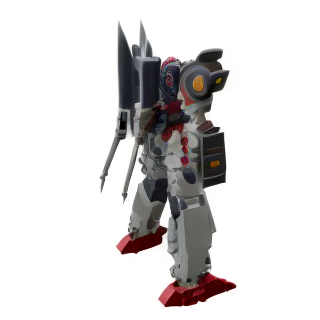
\includegraphics[width=0.13\linewidth]{images/generation_results/sharp-e/gundam/a_gundam_75_steps_batch_0_a_gundam_tile_2.png} &
    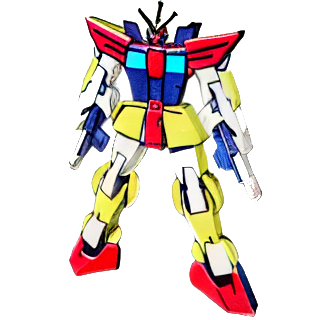
\includegraphics[width=0.13\linewidth]{images/generation_results/zero123/gundam/gundam_tile_0.jpg} & { } & 
    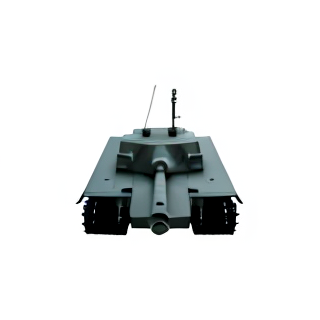
\includegraphics[width=0.13\linewidth, trim=20 50 20 50, clip]{images/generation_results/sharp-e/tank/a_battle_tank_75_steps_batch_0_a_battle_tank_tile_4.png} &
    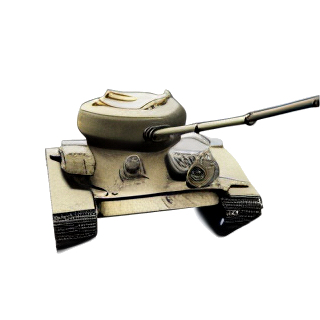
\includegraphics[width=0.13\linewidth, trim=0 20 0 20, clip]{images/generation_results/zero123/tank/tank_tile_0.png} & { } & 
    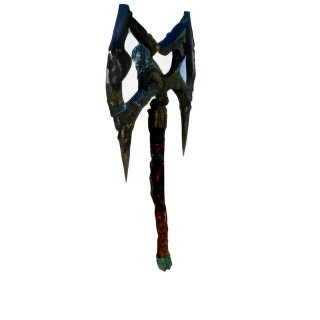
\includegraphics[width=0.13\linewidth]{images/generation_results/sharp-e/axe/2_250_steps_batch_0_a_battle_axe_made_out_of_glass_tile_0.png} &
    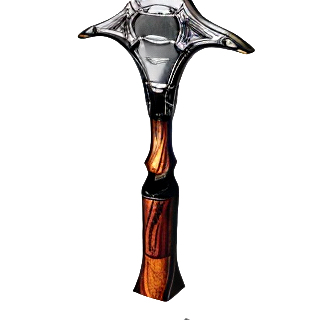
\includegraphics[width=0.13\linewidth]{images/generation_results/zero123/glass_axe/glass_axe_14_tile_0.jpg}
    \\
    %
    \raisebox{20pt}{\rotatebox[origin=c]{90}{View 2}} &
    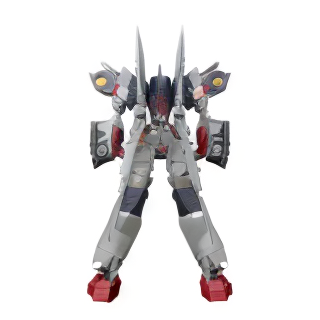
\includegraphics[width=0.13\linewidth]{images/generation_results/sharp-e/gundam/a_gundam_75_steps_batch_0_a_gundam_tile_1.png} &
    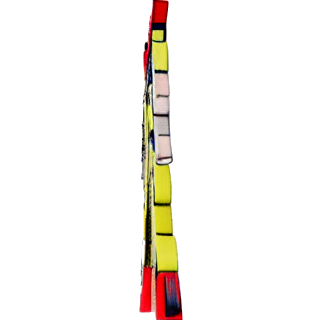
\includegraphics[width=0.13\linewidth]{images/generation_results/zero123/gundam/gundam_tile_1.jpg} & { } & 
    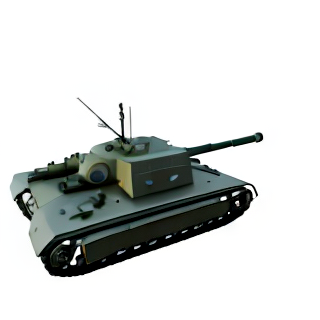
\includegraphics[width=0.13\linewidth, trim=0 0 0 60, clip]{images/generation_results/sharp-e/tank/a_battle_tank_75_steps_batch_0_a_battle_tank_tile_2.png} &
    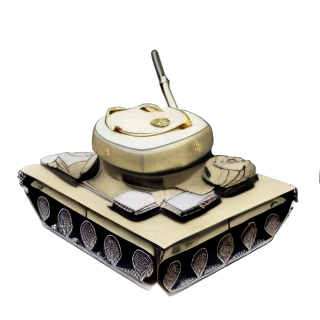
\includegraphics[width=0.13\linewidth, trim=0 0 0 20, clip]{images/generation_results/zero123/tank/tank_tile_4.png} & { } & 
    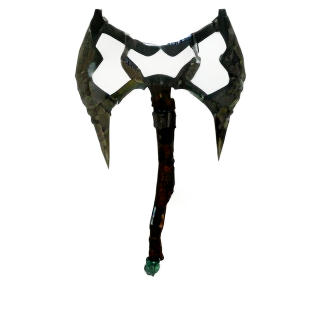
\includegraphics[width=0.13\linewidth]{images/generation_results/sharp-e/axe/2_250_steps_batch_0_a_battle_axe_made_out_of_glass_tile_4.png} &
    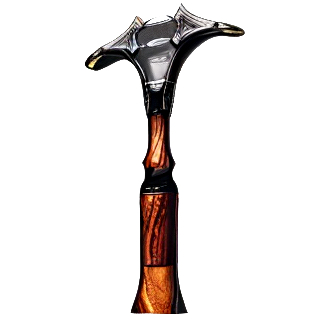
\includegraphics[width=0.13\linewidth]{images/generation_results/zero123/glass_axe/glass_axe_14_tile_3.jpg} \\
    %
    & \multicolumn{1}{c}{Ours} & \multicolumn{1}{c}{Zero123++} & { } & \multicolumn{1}{c}{Ours} & \multicolumn{1}{c}{Zero123++} & { } & \multicolumn{1}{c}{Ours} & \multicolumn{1}{c}{Zero123++} \\
     
\end{tabular}
}
\vspace{-8pt}
\caption{
Text-to-MultiView qualitative results. Our method generates a multi-view set by creating a 3D object with Shap-E and refining it with Sharp-It. In contrast, Zero123++ first generates a single image with Stable Diffusion, then produces a multi-view set conditioned on that image. This approach leads to geometric artifacts, such as flatness (gundam) and the Janus problem (tank). Leveraging Shap-E's 3D knowledge, our method yields high-quality, coherent objects. Additional 3D renderings of these results are provided in the supplemental.
}
\vspace{-12pt}
\label{fig:text-to-3d}
\end{figure*}